\documentclass{chi-ext}
% Please be sure that you have the dependencies (i.e., additional LaTeX packages) to compile this example.
% See http://personales.upv.es/luileito/chiext/

\copyrightinfo{
  Copyright is held by the author/owner(s).\\
  This is a generic SIGCHI \LaTeX\ template sample.\\
  The corresponding ACM copyright statement must be included.
}

\title{HCI-Projektbericht Draw-to-Clipboard}

\numberofauthors{8}
% Notice how author names are alternately typesetted to appear ordered in 2-column format;
% i.e., the first 4 autors on the first column and the other 4 auhors on the second column.
% Actually, it's up to you to strictly adhere to this author notation.
\author{
  \vspace{-1.5em} % lisatolles: The abstract heading should start at the time height on the page as the authors names
  \alignauthor{
  	\textbf{Constantin Gerstberger}\\
  	\affaddr{Theresienstr. 11}\\
  	\affaddr{82131 Gauting, Germany}\\
  	\email{constantin.gerstberger@gmail.com}
  }\alignauthor{
  	\textbf{Sebastian W\"ohrl}\\
  	%\affaddr{123 Author Ave.}\\
  	%\affaddr{Authortown, PA 54321 USA}\\
  	\email{sebastian.woehrl@mytum.de}
  }
  \vfil
  \alignauthor{
  	\textbf{Manfred Schmidbartl}\\
  	\affaddr{123 Author Ave.}\\
  	\affaddr{Authortown, PA 54321 USA}\\
  	\email{author2@anotherco.com}
  }
  \vfil
  \alignauthor{
  	\textbf{Benjamin Schwartz}\\
  	\affaddr{123 Author Ave.}\\
  	\affaddr{Authortown, PA 54321 USA}\\
  	\email{author3@anotherco.com}
  }
  \vfil
  \alignauthor{
  	\textbf{Marcus Vetter}\\
  	\affaddr{Hofheimerstr. 6}\\
  	\affaddr{81245 Muenchen, Germany}\\
  	\email{marcus.vetter@tum.de}
  }
}

% Paper metadata (use plain text, for PDF inclusion and later re-using, if desired)
\def\plaintitle{HCI-Projektbericht Draw-to-Clipboard}
\def\plainauthor{Constantin Gerstberger, Manfred Schmidbartl, Benjamin Schwartz, Marcus Vetter, Sebastian W\"ohrl}
\def\plainkeywords{Mobile Application, HCI, Gesture Interface}
%\def\plaingeneralterms{Documentation, Standardization}

\hypersetup{
  % Your metadata go here
  pdftitle={\plaintitle},
  pdfauthor={\plainauthor},  
  pdfkeywords={\plainkeywords},
  %pdfsubject={\plaingeneralterms},
  % Quick access to color overriding:
  %citecolor=black,
  %linkcolor=black,
  %menucolor=black,
  %urlcolor=black,
}

\usepackage{graphicx}   % for EPS use the graphics package instead
\usepackage{balance}    % useful for balancing the last columns
\usepackage{bibspacing} % save vertical space in references


\begin{document}

\maketitle

\begin{abstract}
In this sample we describe the formatting requirements for various SIGCHI related submissions 
and offer recommendations on writing for the worldwide SIGCHI readership. 
%Do not change the page size or page settings.
Please review this document even if you have submitted to SIGCHI conferences before, 
some format details have changed relative to previous years.
\end{abstract}

\keywords{\plainkeywords}



% =============================================================================
\section{Problemstellung und Motivation}
% =============================================================================
Zwar ist das papierlose Büro in vielen Fällen noch immer eine Utopie, doch zumindest die papierlose Vorlesung wird für Studenten immer mehr zur Realität. Vorlesungsmitschriften und Notizen auf Papier werden immer seltener, stattdessen wird das eigene Notebook als Schreibutensil verwendet. Doch noch immer besitzen die wenigsten Notebooks einen Touchscreen, was das Mitschreiben von Zeichnungen oder komplizierten Formeln zur Qual macht. 
Bedenkt man jedoch, dass in der heutigen Zeit Smartphones vor allem bei Studenten ein nicht mehr wegzudenkender Ausrüstungsgegenstand sind, und diese praktisch immer einen Touchscreen besitzen, war das für uns die Motivation, die Geräte Notebook und Smartphone miteinander zu verbinden um die Aufgabe Digitale Vorlesungsmitschrift besser zu lösen.

Erreichen wollten wir dies, indem wir eine App für Smartphones entwickeln, die es Nutzern erlaubt, auf dem Smartphone Zeichnungen oder Skizzen anzufertigen und diese dann auf ihr Notebook zu übertragen und dort direkt in eine geöffnete Anwendung wie etwa Microsoft Word einzufügen.


Die Problemstellung lässt sich in mehrere Teile aufgliedern:\\
Zum einen das Anfertigen der Skizze auf dem Smartphone. Hier muss die App die Möglichkeiten einer Zeichen- bzw. Mal-App bieten. Andererseits sollten es nicht zu viele Features sein um den Hauptanwendungszweck nicht aus den Augen zu verlieren.
Der zweite Teil der Problemstellung dreht sich um die Übertragung der angefertigten Skizze auf den Laptop. Dabei geht es sowohl um die technische Realisierung (welche Übertragungstechnik) als auch darum die Funktion einfach und komfortabel benutzbar zu machen.
Um diesen letzten Punkt dreht sich auch unsere Studie, in der wir unter anderem untersuchen, wie sich die Übertragung der Skizze vom Smartphone auf den Laptop am benutzerfreundlichsten auslösen lässt.
%% TODO: Noch mehr Labern

Um uns über eine repräsentative Nutzung unseres Systems klar zu werden und damit gleichzeitig mögliche Features und interessante Gebiete für unsere Studie zu finden, haben wir uns ein Szenario anhand einer konkreten Persona überlegt. 

Doch zuerst hatten wir uns in diesem Rahmen Gedanken zu möglichen Zielgruppen gemacht: \\
Als primäre Zielgruppe lassen sich Teilnehmer von Seminaren, Konferenzen, Vorlesungen definieren, welche daran interessiert sind eigene komplexe Gedanken sowie Notizen zum Vortrag in grafischer Form festzuhalten und dynamisch in Officeprogrammen einzubinden.
Aufgrund der Grundannahmen für unsere Anwendung lässt sich für diese Zielgruppe als Eingrenzungsbedingung definieren, dass der Gruppe ein Laptop/Tablet sowie ein Smartphone zur Verfügung stehen muss. 
Es fällt dabei auf, dass die sich ergebende Gruppe sehr heterogen ausfällt. Die Anwendung ist für unterschiedliche Altergruppen (Schüler, Studenten, Geschäfftsmänner, Wissenschaftler... ) , unterschiedliche Themenbereiche (technische, sozialwisschenschaftliche, künstlerische ...) sowie Personengruppen mit unterschiedlichen technischen Vorkentnissen sinnvoll einsetzbar.

Eine Gemeinsamkeit lässt sich jedoch finden: Das Motiv und somit der praktische Nutzen für die Verwendung des Programm ist hingegen für alle Teilgruppen gleich und vereint diese.
Dieses Motiv lässt sich wie folgt formulieren:\\
Die Nutzer haben ein Bedürfnis die vermittelten Inhalte organisiert und verständlich aufzubereiten. Die Anwendung ermöglicht dabei komplexe grafische Inhalte des Vortrages effizient mit den bereits gegebenen technischen Mitteln mitzunotieren.

Auf Basis dieser heterogenen aber doch wieder homogenen Zielgruppe haben wir uns für unser Szenario als konkrete Persona einen Mathe-Studenten namens Marko überlegt.


% =============================================================================
\section{Szenario}
% =============================================================================
Das im folgenden beschrieben Nutzerszenario beschreibt eine typische Interkation mit unserer Android Applikation während einer Vorlesung:


Marko, ein Mathe-Student, schreibt seine Notizen per Tastatur mit. Marko besitzt kein Bamboo oder ähnliche Zeichenpads um Skizzen per Hand in das Notebook zu übertragen. Nun kommt es zu dem Punkt, an dem der Professor im Fach Mathematik III die Folgerung der Cauchyschen Integralformel für Kreisschreiben an die Tafel schreibt, welche nicht mehr per Tastatur abzubilden ist.

\begin{figure}
  \centering
  \includegraphics[width=\linewidth]{img/szenario/szenario_1.jpg}
  \caption{Basic user interface (startscreen)}
  \label{fig:mockup_startscreen}
\end{figure}

Also nimmt Marko sein Smartphone aus der Tasche, welches mit dem Internet verbunden ist, um nun mit diesem die Skizzen abmalen zu können. Zudem öffnet er unsere Anwendung am Notebook (z.B. Tray-Icon), welche ebenfalls eine Internetverbindung besitzt. Er klickt auf das Tray-Icon (rechte Maustaste) und wählt dort Pairen mittels QR Code aus. In der Android App gibt es, wenn man den Menü Button drückt ebenfalls eine Option „pairen“. Marko wählt diese Funktion aus und bekommt eine Liste mit Möglichkeiten zum Verbinden zwischen Smartphone und Computer angezeigt. Er wählt QR-Code aus und kann nun mit seiner Handykamera den QR Code vom Bildschirm abscannen. Nachdem der QR-Code eingescannt wurde, stellen das Notebook und das Smartphone im Hintergrund eine Verbindung her. Am PC erkennt man dies am Farbenwechsel des Tray-Icons. Am Smartphone erfolgt keine Benachrichtigung um Marko nicht abzulenken und ihm die größtmögliche Fläche für seine Eingaben zu bieten. Wenn das Tray-Icon auf grün wechselt, dann sind Smartphone und Notebook gekoppelt. Der Kopplungsvorgang kann natürlich auch über USB, Bluetooth oder ähnliche Techniken erfolgen.\\
Marko kann nun die Skizze von der Tafel übernehmen. Dies bewerkstelligt er über das Smartphone, indem er von der Anwendung ein Art weißes Blatt Papier präsentiert bekommt und dort mittels Finger oder Stift Notizen und Skizzen eingeben kann.

\begin{figure}
  \centering
  \includegraphics[width=\linewidth]{img/szenario/szenario_2.jpg}
  \caption{Basic user interface (startscreen)}
  \label{fig:mockup_startscreen}
\end{figure}
 
 Um diese Skizze an den PC zu übertragen, kann nun entweder der Menüpunkt gewählt werden oder man kann sein Smartphone schnell in eine Richtung bewegen (ähnlich einem Werf-Vorgang). Diese Bewegung kann mithilfe der Beschleunigungssensoren wahrgenommen werden. Marko entscheidet sich für die traditionelle Variante und drückt den Button.
Das Smartphone zeigt den erfolgreichen Vorgang durch eine Vibration an und zeigt einen grünen Pfeil im Bildschirm. Zudem wird der Zeichenbereich geleert um direkt eine neue Skizze zu beginnen. Falls es zu einer fehlerhaften Erkennung der Werf-Geste gekommen ist, gibt es die Möglichkeit die Skizze wiederherzustellen, indem man den Menü Button drückt und dort „Skizze wiederherstellen“ wählt.

\begin{figure}
  \centering
  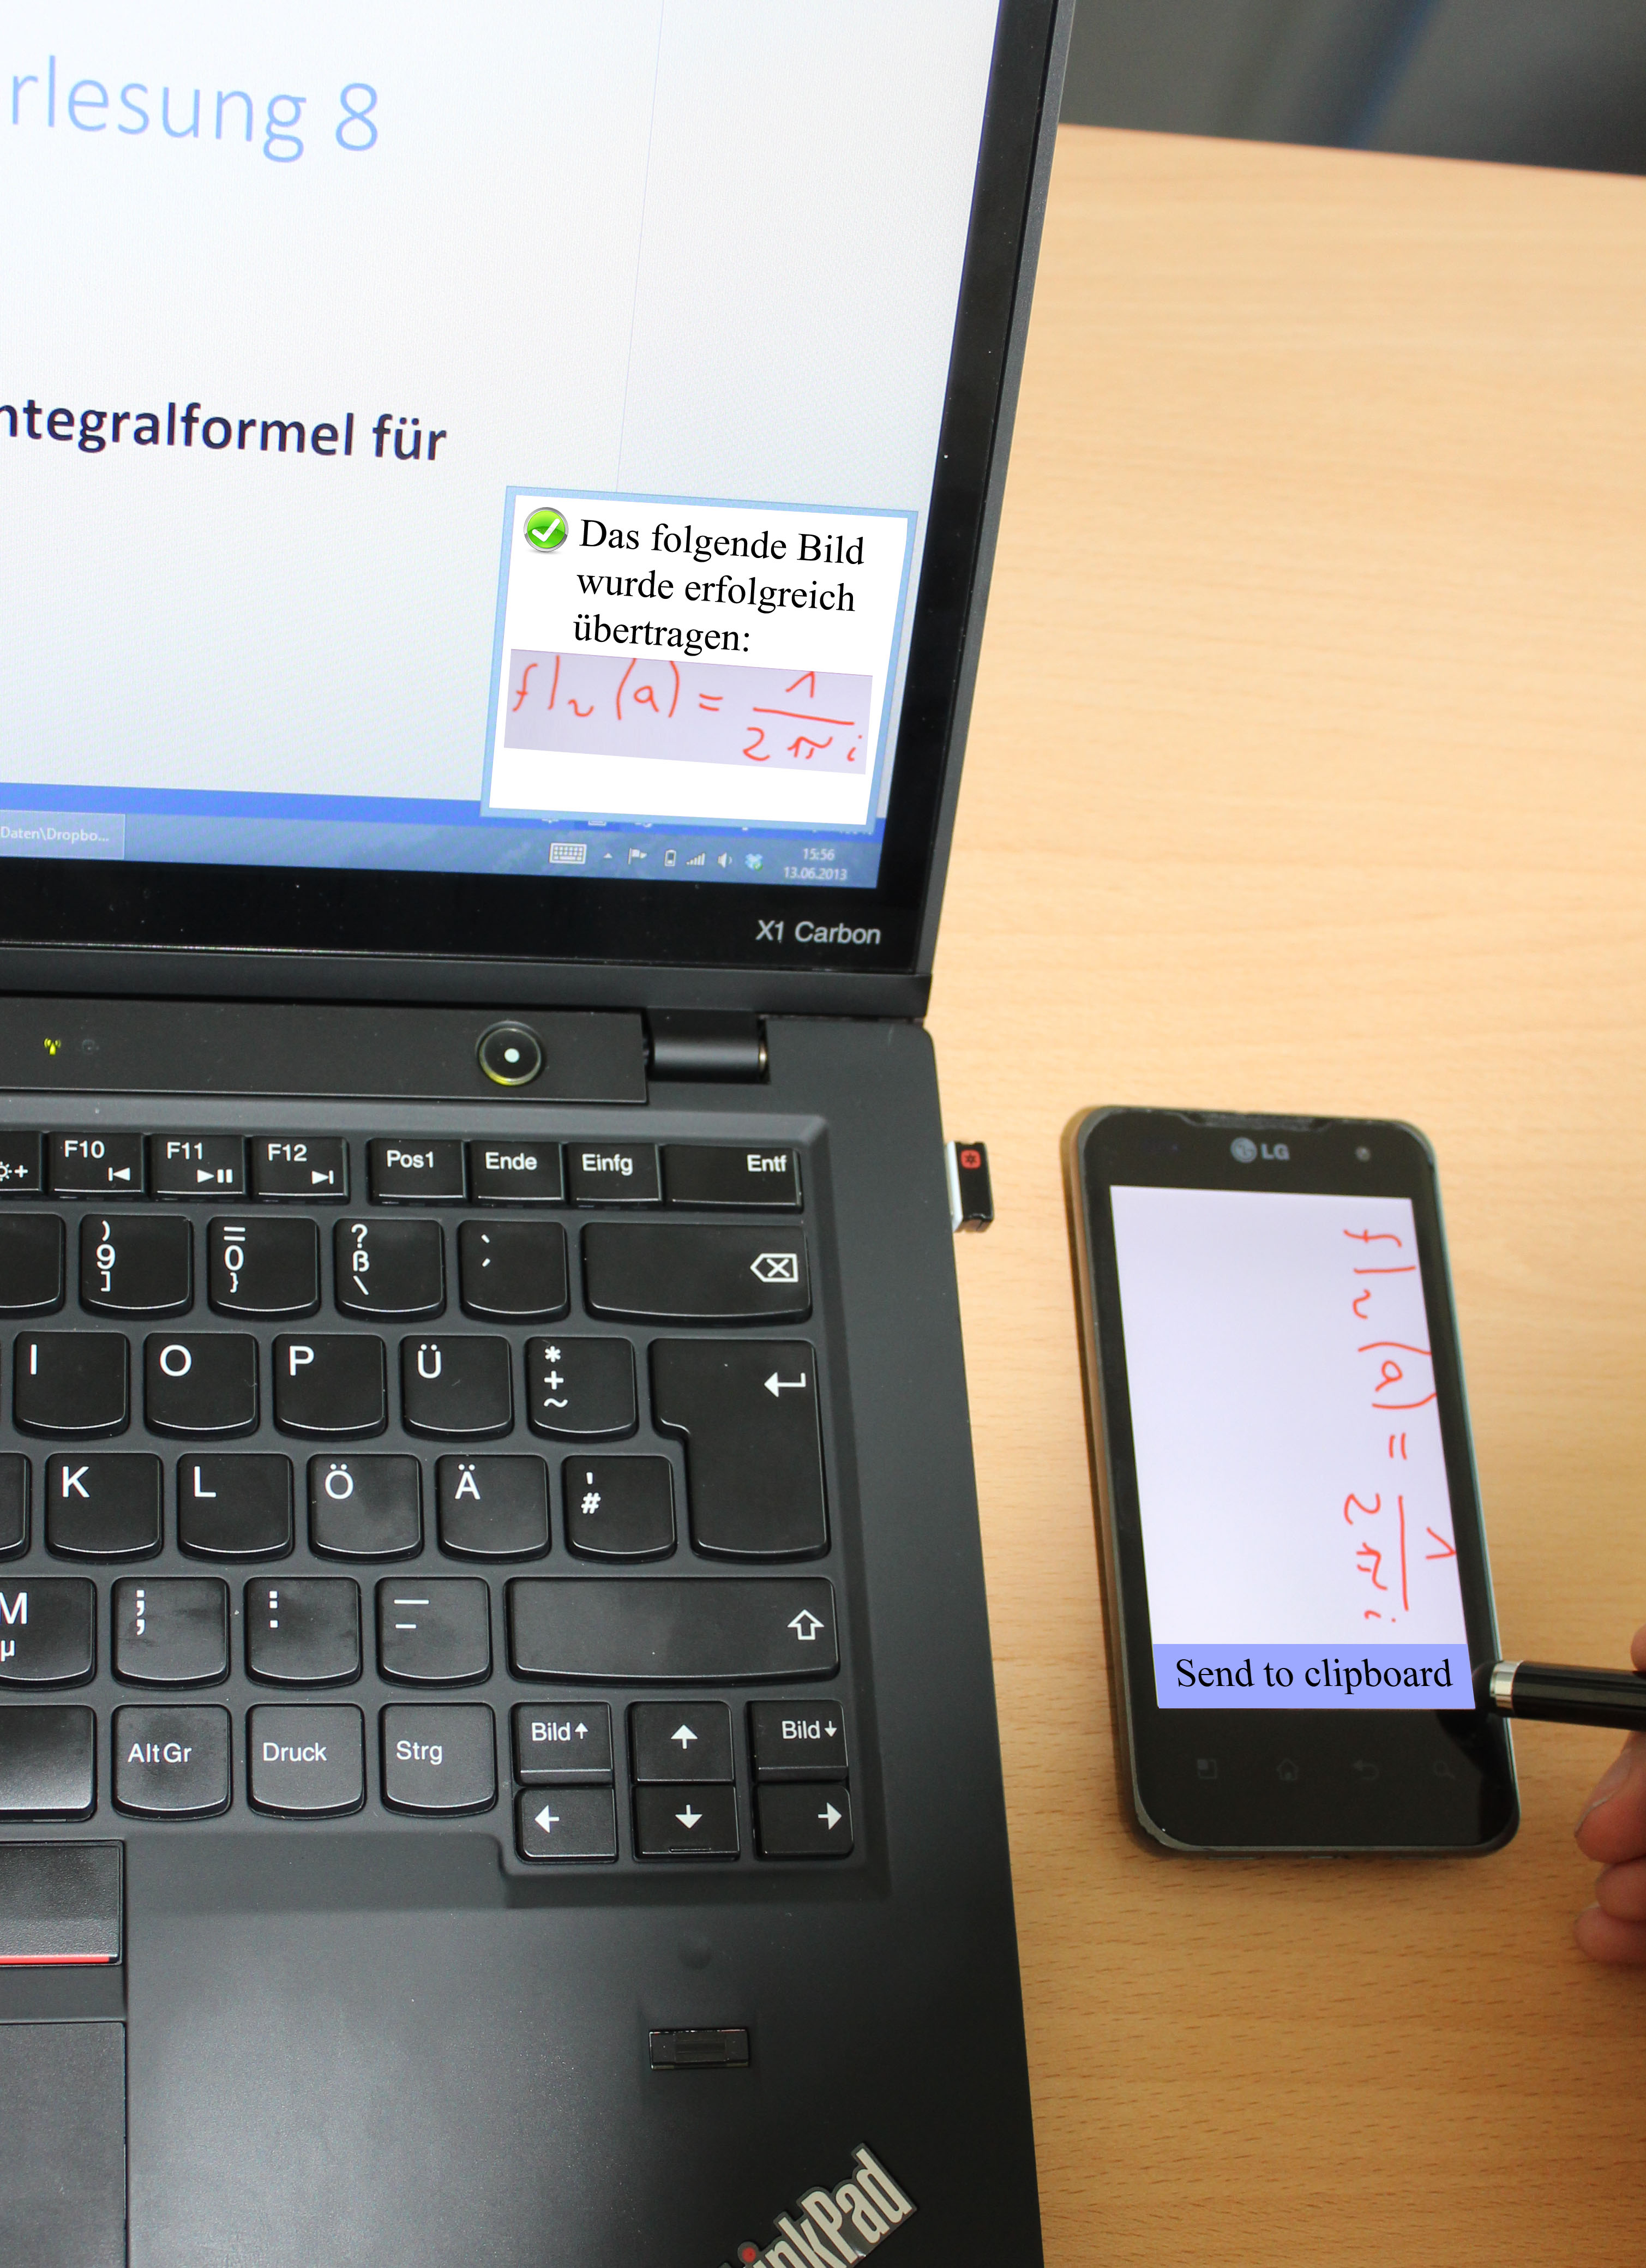
\includegraphics[width=\linewidth]{img/szenario/szenario_3.jpg}
  \caption{Basic user interface (startscreen)}
  \label{fig:mockup_startscreen}
\end{figure}
 
Am Notebook wird durch einen Hinweis im Tray-Bereich angezeigt, dass Marko die Skizze nun am Notebook bereitgestellt worden ist. Sie ist automatisch in der Zwischenablage des Betriebssystems abgelegt worden, damit Marko die Skizze sofort in seine Notizen einfügen kann. 
Die anderen Studenten im Saal haben natürlich bemerkt, dass Marko die Skizze nun digital verfügbar hat und würden diese auch gerne auf ihrem PC haben. Marko kann nun einfach in der Anwendung am Notebook über das Tray-Icon auswählen, dass er eine Skizze per E-Mail verschicken möchte. Dort gibt es zwei Möglichkeiten, einmal im Standard E-Mail Programm eine vorgefertigte E-Mail zu öffnen, wo die Skizze angehangen ist oder sie direkt an eine vordefinierte Gruppe von Studenten zu verschicken. Marko hat seine Mathe-Lerngruppe schon abgespeichert und kann nun die Skizze direkt per Rundmail an seine Kommilitonen schicken.

% =============================================================================
\section{Low-fidelity Prototyp}
% =============================================================================
\begin{itemize}
	\item {\textbf{Zeigertool:} Kann verwendet werden um zu zoomen oder die Zeichenfläche nach links, rechts, oben oder unten zu verschieben}
	\item {\textbf{Stift:} Mit dem Stift kann auf der Zeichenfläche gezeichnet werden.}
	\item {\textbf{Farbwahl:} Hier kann eine Stiftfarbe ausgewählt werden}
	\item {\textbf{Stiftdicke:} Hier kann die Dicke des Stiftes ausgewählt werden}
	\item {\textbf{Löschen:} Hier kann die komplette Zeichenfläche geleert werden.}
	\item {\textbf{Senden:} Hier kann die erstellte Zeichnung an das Clipboard des PCs gesendet werden.}
\end{itemize}

\begin{figure}
  \centering
  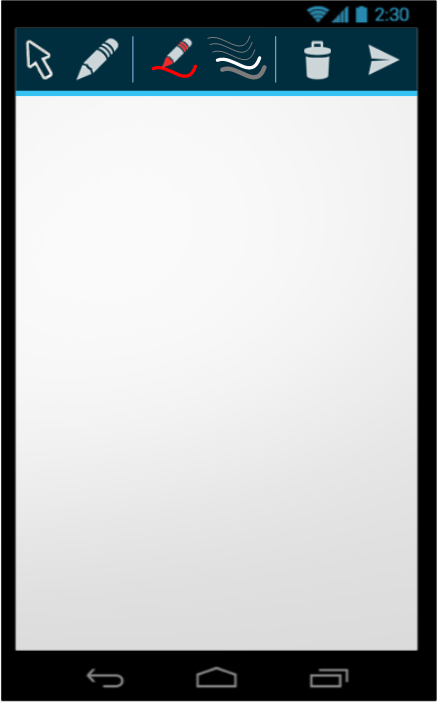
\includegraphics[width=\linewidth]{img/android/mockup_startscreen.png}
  \caption{Basic user interface (startscreen)}
  \label{fig:mockup_startscreen}
\end{figure}

\begin{figure}
  \centering
  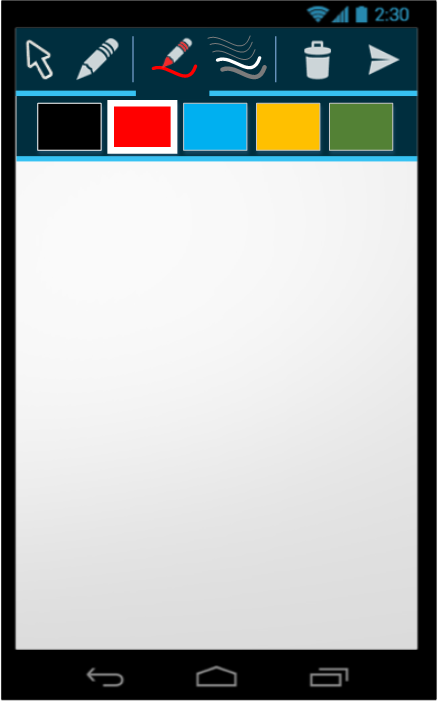
\includegraphics[width=\linewidth]{img/android/mockup_color.png}
  \caption{Select a color)}
  \label{fig:mockup_color}
\end{figure}

\begin{figure}
  \centering
  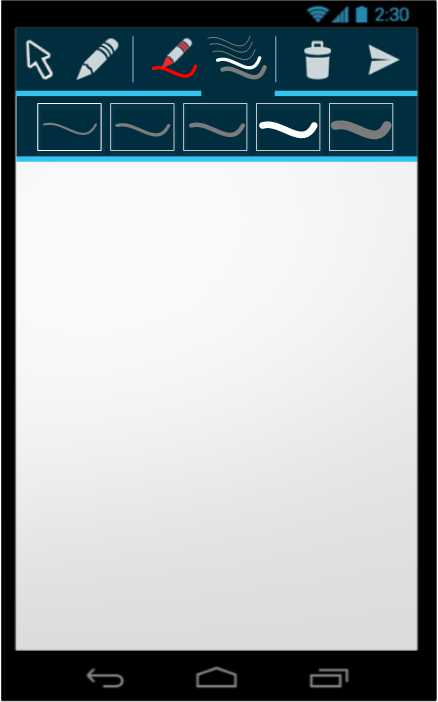
\includegraphics[width=\linewidth]{img/android/mockup_pen.png}
  \caption{Select a pen}
  \label{fig:mockup_pen}
\end{figure}

% =============================================================================
\section{Ergebnisse der Studie}
% =============================================================================
Blubb
% TODO: Bla bla bla

% =============================================================================
\section{Diskussion}
% =============================================================================
Bei der Studie hat sich unter anderem gezeigt, dass, entgegen unserer Erwartungen, die meisten Nutzer für das Auslösen der Übertragung zum Laptop keine Bewegungsgeste mit dem Smartphone sondern eher einen zu betätigenden Button bevorzugen. Dies ist auf den ersten Blick überraschend, zeigen mehrere Studien [TODO] doch ausführlich, dass Bewegungsgesten sehr natürlich sind. Jedoch sind Benutzer von Computern an die seit Jahren praktisch überall eingesetzte Maus- und Tastatur-Steuerung gewöhnt, bei der die Bedienung durch das Drücken von Buttons mit der Maus erfolgt. Diese hat sich auch auf Smartphones übertragen, nur werden die Buttons dort per Touchscreen direkt mit dem Finger bedient. Durch diese jahrelange Gewöhnung sehen geübte Benutzer diese Bedienung wohl als völlig natürlich an und empfinden dann daher auch das Betätigen eines Buttons als einfache und benutzerfreundliche Geste. Bewegungsgesten mit dem Smartphone wären damit eher eine Umstellung, auch wenn der Wow-Effekt natürlich größer wäre als beim Betätigen eines Buttons.
%% TODO: Anpassen an konkrete Ergebnisse der Studie und Erweitern


% =============================================================================
\section{Konklusion}
% =============================================================================
In diesem Paper haben wir unser Projekt Copy-To-Clipboard vorgestellt, das wir im Rahmen der HCI-Vorlesung im Sommersemester 2013 an der Universität Augsburg durchgeführt haben. Dabei haben wir die wirkliche Durchführung des Projekts, also die Implementierung außen vor gelassen, und uns auf die HCI-Aspekte des Projekts beschränkt um den iterativen, nutzerzentrierten HCI-Designprozess zu verstehen und anzuwenden.
% TODO: Bla bla bla



\balance
\bibliographystyle{acm-sigchi}
\bibliography{sample}

\end{document}